\subsection{Fast Fourier Transform}
\subsubsection{Introducción al algoritmo}
El algoritmo de Cooley-Tukey, nombrado así por J.W. Cooley y John Tukey, es el algoritmo más común de transformada rápida de Fourier. El algoritmo expresa la transformada discreta de Fourier (DFT) de tamaño de un número compuesto N=N1N2 en términos de transformadas discretas de tamaños N1 y N2, de manera recursiva, para reducir su complejidad a O(N log N) para un número altamente compuesto N(smooth numbers). \\

\begin{center}
    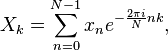
\includegraphics[height=1cm]{images/fft_formula.png}
\end{center}

\subsubsection{Algoritmo de diezmado en el tiempo}

El algoritmo de diezmado en el tiempo de doble radix (decimation-in-time DIT) para la FFT es la forma más simple y común del algoritmo de Cooley–Tukey.
El algoritmo de Radix-2 DIT divide a la transformada discreta de Fourier de tamaño N en 2 transformadas discretas intercaladas (de ahí el nombre de doble radix o Radix-2) de tamaño N/2 en cada etapa recursiva.\\

Este algoritmo calcula inicialmente por separado los índices pares de los impares, nosotros aprovechamos esto para que los índices pares sean calculados por un core mientras los impares eran calculados por otro, de manera de aumentar la velocidad.\\

Este algoritmo es un caso interesante a estudiar debido a que constantemente los cores debían sincronizarse para trabajar, lo que nos permitió ver cómo se comportaban los diferentes métodos de sincronización con una alta demanda.\\

En la próxima sección de mostrarán resultados de la paralelización de este algoritmo.

\vspace{1cm}
Procesamiento de FFT:
\begin{center}
    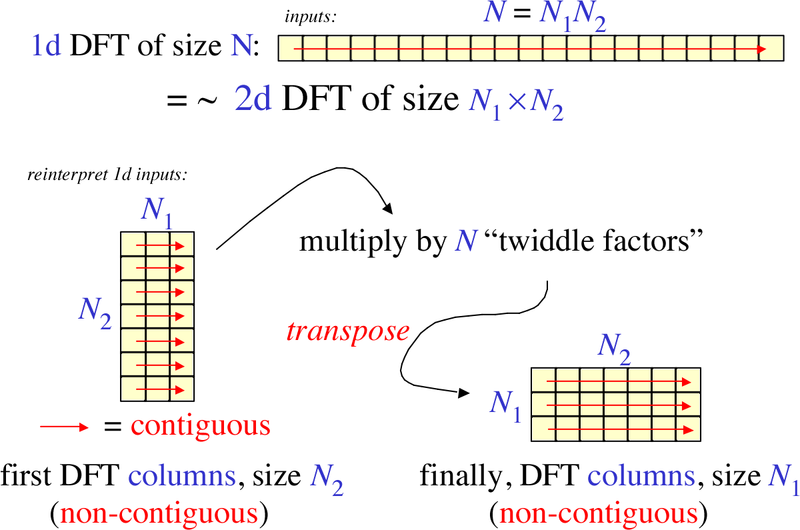
\includegraphics[height=8cm]{images/Cooley-tukey-general.png}
\end{center}

\vspace{1cm}
Sincronización de FFT:
\begin{center}
    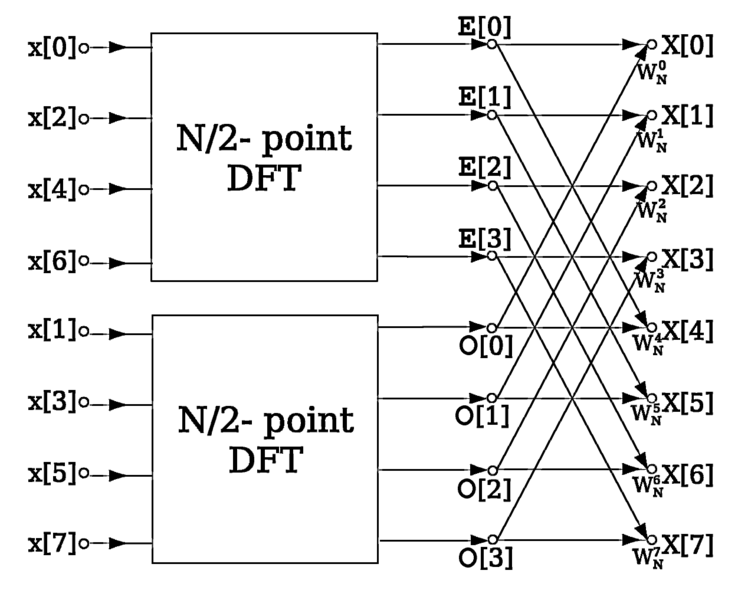
\includegraphics[height=8cm]{images/DIT-FFT-butterfly.png}
\end{center}
